\documentclass[a4paper,leqno]{article}
\usepackage[utf8]{inputenc}
\usepackage{lmodern}
\usepackage{microtype}
\usepackage[inline]{enumitem}

\usepackage{siunitx}
\usepackage{multirow}
\usepackage{subcaption}

\usepackage[english]{babel}
\usepackage[autostyle, english=british]{csquotes}
\MakeOuterQuote{"}

\usepackage{commath}
\usepackage{amsmath}
\usepackage{amsthm}
\usepackage{amssymb}

\usepackage{pgfplots}
\pgfplotsset{compat=1.11}
\usepgfplotslibrary{fillbetween}
\usetikzlibrary{patterns}

\usepackage{hyperref}

\usepackage[margin=1in]{geometry}
\usepackage{changepage}
\usepackage{titlesec}
\titleformat{\section}{\normalfont\Large\bfseries\centering}{Section~\thesection:}{1em}{}

\def\signed #1{{\leavevmode\unskip\nobreak\hfil\penalty50\hskip2em
  \hbox{}\nobreak\hfil(#1)%
  \parfillskip=0pt \finalhyphendemerits=0 \endgraf}}
\newsavebox\mybox
\newenvironment{aquote}[1]
  {\savebox\mybox{#1}\begin{quote}}
  {\signed{\usebox\mybox}\end{quote}}

% Augmented matrices.
\makeatletter
\renewcommand*\env@matrix[1][*\c@MaxMatrixCols c]{%
  \hskip -\arraycolsep
  \let\@ifnextchar\new@ifnextchar
  \array{#1}}
\makeatother

%--------grstep
% For denoting a Gauss' reduction step.
% Use as: \grstep{\rho_1+\rho_3} or \grstep[2\rho_5 \\ 3\rho_6]{\rho_1+\rho_3}
\newcommand{\grstep}[2][\relax]{%
   \ensuremath{\mathrel{
       {\mathop{\longrightarrow}\limits^{#2\mathstrut}_{
                                     \begin{subarray}{l} #1 \end{subarray}}}}}}
\newcommand{\swap}{\leftrightarrow}


\swapnumbers
\numberwithin{equation}{section}
\newtheorem{thm}[equation]{Theorem}
\newtheorem{lem}[equation]{Lemma}
\newtheorem{cor}[equation]{Corollary}
\newtheorem{prp}[equation]{Proposition}
\theoremstyle{definition}
\newtheorem{defn}[equation]{Definition}
\newtheorem{ex}[equation]{Example}
\newtheorem{exercise}[equation]{Exercise}
\newtheorem{alg}[equation]{Algorithm}
\theoremstyle{remark}
\newtheorem{rem}[equation]{Remark}

\newcommand{\df}[1]{\textbf{#1}}
\newcommand{\T}{\mathrm{T}}
\newcommand{\F}{\mathrm{F}}
\newcommand{\IndSet}{\mathbf{I}}

\title{Level Three Systems of Linear Equations}
\author{Alex Elzenaar}
\date{\today}

\begin{document}
\maketitle
\tableofcontents
\section*{Preface}
\subsection*{To the instructor}
These notes are terse and computational --- this is mainly because the underlying theory (elementary linear algebra) is not a part of the
standard L3 curriculum. If you want pretty proofs, these are not the notes for you! I have proved a few of the easier theorems on simultaneous
linear equations, but of course without the proper linear algebra notation the actual inspiration behind the proofs is impenetrable.

A majority of the exercises I have included are standard and often adapted from other texts (e.g. Whipkey, Whipkey, \& Conway's \textit{The Power
of Mathematics}); I have not included a large number of computational problems as almost all are very similar in style and are easily
found either online or in textbooks. A quick search in the University library catalogue reveals a vast number of books on linear programming,
generally located around [519.72].

\subsection*{To the student}
These notes are in much more detail than is actually required for even an excellence at Level 3. Essentially, examiners are looking for your
ability to solve simple computational problems and to show geometric and/or contextual understanding. While this material is actually very
applicable to industrial applications (e.g. in economics or biology), it is very dry as we do not have time to go off on a tangent to actually
discuss the ideas behind it. As such, these are perhaps the most boring topics presented at this level; if you are actually interested in the
theory and the mathematics behind the techniques, I recommend picking up a book on linear algebra instead.

\titleformat{\section}{\clearpage\titlerule[0.8pt]\vspace{0.5ex}\normalfont\Large\bfseries\centering}{Section~\thesection:}{1em}{}[{\titlerule[0.8pt]}]
\let\oldsection\section
\renewcommand\section{\clearpage\oldsection}
\section{Introduction}
\begin{center}
  \itshape\parbox{0.8\textwidth}{
    Anna, an American, empties her purse and finds that it contains only nickels (worth 5 cents each) and dimes (worth 10 cents each). If she has a total
    of 7 coins and they have a combined value of 45 cents, how many of each coin does she have?
  }
\end{center}

Situations like this often come up when solving problems --- we have two variables (the total amount of each coin), and two linear equations that
they satisfy:
\begin{equation}
  \begin{cases}
    n + d = 7\\
    5n + 10d = 45.
  \end{cases}
\end{equation}

Our goal in this standard is to come up with a procedure for deciding if there are any solutions of such a linear system of equations, and for finding
those solutions if they do exist.

We will begin by formalising the terms which we will be using throughout this standard.

\begin{defn}[Linear equation]
  A \df{linear equation} in $ n $ variables $ x_1 $, $ x_2 $, ..., $ x_n $ is an equation of the form
  \begin{displaymath}
    a_1 x_1 + a_2 x_2 + \cdots + a_n x_n = b
  \end{displaymath}
  for suitable constants $ a_1 $, $ a_2 $, ..., $ a_n $, and $ b $.
\end{defn}

For example, $ 2x + 3y = 3 $ is a linear equation; $ 37x^2 + 23y + 4 = 2 $ is not (because the variable $ x $ is squared); $ \sin x = 3 $ is
not (because $ \sin x $ is not in the given form, and cannot be put into the given form).

\begin{defn}[Linear system of equations]
  A \df{linear system of equations} is a set of linear equations in $ n $ variables $ x_1 $, $ x_2 $, ..., $ x_n $. A \df{solution} of the
  linear system is a set of values for each variable such that every equation is satisfied.
\end{defn}

For example, the system
\begin{equation}
  \begin{cases}
    x + y = 2\\
    2x + 2y + z = 4
  \end{cases}
\end{equation}
has the solution $ (x,y,z) = (1,1,0) $.

\section{Graphing Linear Systems}
\begin{center}
  \emph{``When I use a word," Humpty Dumpty said in a rather scornful tone, ``it means just what I choose it to mean --- neither more nor less." } --- Lewis Carroll
\end{center}
Since each equation is linear, we can easily graph them. We will begin by looking at systems of two variables only, since we can graph
these on a plane.

\begin{ex}
  Consider Anna's system of equations from above,
  \begin{equation}
    \begin{cases}
      n + d = 7\\
      5n + 10d = 45.
    \end{cases}
  \end{equation}
  We can rearrange these to be easier to solve:
  \begin{equation}
    \begin{cases}
      n = 7 - d\\
      n = 9 - 2d,
    \end{cases}
  \end{equation}
  and we can graph these:
  \begin{center}
    \fbox{\begin{tikzpicture}
      \begin{axis}[
        axis lines = center,
        xlabel = $ d $,
        ylabel = $ n $
      ]
        \addplot[domain = 0:5, color = green, samples=100] {7 - x};
        \addplot[domain = 0:5, color = red, samples=100] {9 - 2*x};
      \end{axis}
    \end{tikzpicture}}
  \end{center}
  It follows that there is a unique solution to this system: the point of intersection of the two lines, namely $ (d,n) = (2,5) $.
\end{ex}

\begin{ex}
  Now, consider the following system:
  \begin{equation}
    \begin{cases}
      3x + 2y = 2\\
      6x + 4y = 7.
    \end{cases}
  \end{equation}
  Rearranging to make $ y $ the subject, we have
  \begin{gather*}
    y = \frac{1}{2}(2 - 3x)\\
    y = \frac{1}{4}(7 - 6x).
  \end{gather*}
  \begin{center}
    \fbox{\begin{tikzpicture}
      \begin{axis}[
        axis lines = center,
        xlabel = $ x $,
        ylabel = $ y $
      ]
        \addplot[domain = 0:5, color = orange, samples=100] {0.5*(2 - 3*x)};
        \addplot[domain = 0:5, color = blue, samples=100] {0.25*(7 - 6*x)};
      \end{axis}
    \end{tikzpicture}}
  \end{center}
  From this graph, we can see that the two lines are parallel and hence the system has no solution. We can also prove this algebraically: note
  that the second equation in \ref{eqn:nosoln} implies that $ 3x + 2y = 7/2 $, which contradicts the first.
\end{ex}

\begin{ex}
  For a third example, let us ponder
  \begin{equation}\label{eqn:nosoln}
    \begin{cases}
      3x - 2y = 4\\
      4y - 6x = -8.
    \end{cases}
  \end{equation}
  Rearranging and graphing:
  \begin{center}
    \fbox{\begin{tikzpicture}
      \begin{axis}[
        axis lines = center,
        xlabel = $ x $,
        ylabel = $ y $
      ]
        \addplot[domain = 0:5, color = black, samples=100, ultra thick] {-0.5*(4 - 3*x)};
        \addplot[domain = 0:5, color = red, samples=100, dotted, ultra thick] {0.25*(-8 + 6*x)};
      \end{axis}
    \end{tikzpicture}}
  \end{center}
  In this example, the two equations conincide everywhere and so there are an infinite number of solutions; you should
  verify that $ (2t, 4-3t) $ is a solution for every possible value of $ t $.
\end{ex}

These examples suggest that (for two variables, anyway) there are three possibilities:
\begin{itemize}
  \item A system can have no solutions (it can be \df{impossible}).
  \item A system can have exactly one solution.
  \item A system can have infinitely many solutions.
\end{itemize}
We will prove this in the next section.

\subsection*{Exercises}
\begin{enumerate}
  \item For the following situations, translate the situations into systems of simultaneous equations. \emph{Do not solve the resulting
        systems!}
    \begin{enumerate}
      \item Goldie has twice as many red blocks as blue blocks. The total number of blocks that she has is three times the number of
            blue blocks that she has. How many of each type of block does she have?
      \item Adam breeds chickens and ducks. Last month, he sold 50 chickens and 30 ducks for \$550. This month, he sold 44 chickens
            and 36 ducks for \$532. How much does he sell each bird for?
      \item Emma is comparing telecom companies. Phoneworld has an initial \emph{monthly} cost of \$30, and then charges 5 cents per minute
            of calling. PhoneCity has an initial \emph{yearly} cost of \$200, and charges 20 cents per minute of calling. How many minutes
            per year must Emma be on the telephone for both plans to cost her exactly the same?
      \item Jack rides his bicycle at 15 kilometres per hour; Rowan rides his bicycle at 17 kilometres per hour. They are initially 18
            kilometres apart when they start to ride directly towards each other. How far from Jack's starting point do they meet?
    \end{enumerate}
  \item Graph the following systems of equations. How many solutions does each system have?
    \begin{center}
      \hspace*{\fill}\begin{enumerate*}
        \item
          $ \displaystyle
            \begin{cases}
              2x + 3y = 2\\
              7x - 14y = 7.
            \end{cases}
          $\hspace*{\fill}
        \item
          $ \displaystyle
            \begin{cases}
              x + y = 2\\
              x + y = 4.
            \end{cases}
          $\hspace*{\fill}
        \item
          $ \displaystyle
            \begin{cases}
              x - 3y = 2\\
              2x - 6y = 4.
            \end{cases}
          $\hspace*{\fill}
      \end{enumerate*}
    \end{center}
  \item Consider the system
        \begin{equation*}
          \begin{cases}
            x + y = 2\\
            4x + 4y = n.
          \end{cases}
        \end{equation*}
        Is it possible to pick any value of $ n $ such that this system has a unique solution?
  \item Use a computerised graphing system (such as GeoGebra) to graph the following systems in three variables. Make a conjecture
        about the possible number of solutions for a system of equations with three variables.
    \begin{center}
      \hspace*{\fill}\begin{enumerate*}
        \item
          $ \displaystyle
            \begin{cases}
              - x + y + z = 1\\
              x - y + z = 1\\
              x + y - z = 1.
            \end{cases}
          $\hspace*{\fill}
        \item
          $ \displaystyle
            \begin{cases}
              - x + y + z = 1\\
              x - y - z = 1\\
              -x + y - z = 1.
            \end{cases}
          $\hspace*{\fill}
        \item
          $ \displaystyle
            \begin{cases}
              2x + y - z = 4\\
              4x + 2y - 2z = 5\\
              8x - 4y - 4z = 16.
            \end{cases}
          $\hspace*{\fill}
      \end{enumerate*}
    \end{center}
\end{enumerate}

\section{The Main Theorem on Linear Equalities}
\begin{center}
  \emph{Never underestimate the power of a theorem that counts something.}  --- Unknown.
\end{center}
The goal in this section is to prove the following theorem that we observed in the last section:
\begin{thm}[Main Theorem on Linear Equalities]\ \\
  Given any system of linear equations, we have three possibilities:
  \begin{itemize}
    \item The system is inconsistent (that is, it has no solutions).
    \item The system is consistent and has a single unique solution.
    \item The system has infinitely many solutions.
  \end{itemize}
\end{thm}

The proof is quite technical, however, so readers who wish to skip it may do so. We begin by proving the theorem for the two smallest cases (systems
of a single variable, and systems of two variables) in the following two lemmata --- they are not actually necessary for our main proof, but they are
much easier to understand.

\begin{lem}
  Consider any system of a single variable. Then we have exactly two possibilities:
  \begin{itemize}
    \item The system is inconsistent (that is, it has no solutions).
    \item The system is consistent and has a single unique solution.
  \end{itemize}
\end{lem}
\begin{proof}
  A system of a single variable will look like
  \begin{equation}
    \begin{cases}
      a_1 x = b_1\\
      a_2 x = b_2\\
        \hspace{0.15em}\qquad\vdots\\
      a_m x = b_x.
    \end{cases}
  \end{equation}

  It is clear that it is possible for such a system to have either no solutions (e.g. take $ a_1 = 0 $ and $ b_1 = 1 $) or exactly one solution. Now,
  suppose that the system has two solutions $ x $ and $ x' $. Then, in particular, we have $ a_1 x = b_1 $ and $ a_1 x' = b_1 $; so $ x = x' $.
\end{proof}

\begin{lem}
  Consider any system of two variables. Then we have exactly three possibilities:
  \begin{itemize}
    \item The system is inconsistent (that is, it has no solutions).
    \item The system is consistent and has a single unique solution.
    \item The system has infinitely many solutions.
  \end{itemize}
\end{lem}
\begin{proof}
  It is clear that it is possible for such a system to have either no solutions, exactly one solution, or at least two solutions. Now,
  suppose that the system has two distinct solutions $ (x,y) $ and $ (x',y') $. Let $ t $ be any number, and suppose that $ a_i x + b_i y = c_i $ is any equation
  in the system. Then $ \left(t, \frac{y - y'}{x - x'} t + \frac{c_i}{b_i}\right) $ is a solution:
  \begin{align*}
    a_i t + b_i \left(\frac{y - y'}{x - x'} t + \frac{c_i}{b_i}\right) &= a_i t + t\frac{b_i y - b_i y'}{x - x'} + c_i\\
                                                                       &= a_i t + t\frac{(c_i - a_i x) - (c_i - a_i x')}{x - x'} + c_i\\
                                                                       &= a_i t + t\frac{c_i - c_i + a_i x' - a_i x}{x - x'} + c_i\\
                                                                       &= a_i t + t\frac{a_i(x' - x)}{x - x'} + c_i\\
                                                                       &= a_i t - a_i t + c_i = c_i.
  \end{align*}
  Hence, if we have at least two distinct solutions, then we have an infinite number of solutions (one for each $ t $) --- and we are done.
\end{proof}

Now for the killing blow. The proof we give here will probably seem to be pulled out of thin air (i.e. there seems to be no motivation --- how
did I come up with it?). The reason for this is that the standard proof of this uses a branch of mathematics known as \emph{linear algebra}. I
have translated the proof from the notation of that area of study into the kind of arithmetical algebra that you see below.

Essentially the idea is the same as for the $ n = 2 $ case in the lemma above; we note that $ (x_1 - x'_1, ..., x_n - x'_n) $ is almost a solution,
in the sense that it makes all the constant terms zero (this set of values is in the \df{nullspace} of our system), and then we add on one of our original
solutions to get the correct constant terms.

\begin{proof}[Proof of the main theorem]
  Let us consider a system of $ n $ variables:
  \begin{equation}
    \begin{cases}
      {a_1}_1 x_1 + {a_1}_2 x_2 + \cdots + {a_1}_{n - 1} x_{n - 1} + {a_1}_n x_n = b_1\\
      {a_2}_1 x_1 + {a_2}_2 x_2 + \cdots + {a_2}_{n - 1} x_{n - 1} + {a_2}_n x_n = b_2\\
        \hspace{0.15em}\qquad\vdots\\
      {a_m}_1 x_1 + {a_m}_2 x_2 + \cdots + {a_m}_{n - 1} x_{n - 1} + {a_m}_n x_n = b_m
    \end{cases}
  \end{equation}
  Suppose that we have two distinct solutions, $ (x_1, ..., x_n) $ and $ (x'_1, ..., x'_n) $; let $ t $ be a number, and consider
  $ (x_1 + t(x_1 - x'_1), x_2 + t(x_2 - x'_2), ..., x_n + t(x_n - x'_n)) $. Then we see that this is a solution to the $ i$th equation
  in the system:
  \begin{align*}
    &{a_i}_1 (x_1 + t(x_1 - x'_1)) + \cdots + {a_i}_n (x_n + t(x_n - x'_n))\\
    &\qquad = {a_i}_1 x_1 + {a_i}_1 t(x_1 - x'_1) + \cdots + {a_i}_n x_n + {a_i}_n t(x_n - x'_n)\\
    &\qquad = ({a_i}_1 x_1 + \cdots + {a_i}_n x_n) + t({a_i}_1 (x_1 - x'_1) + \cdots + {a_i}_n (x_n - x'_n))\\
    &\qquad = b_i + t[({a_i}_1 x_1 + \cdots + {a_i}_n x_n) - ({a_i}_1 x'_1 + \cdots + {a_i}_n x'_n)]\\
    &\qquad = b_i + t[b_i - b_i] = b_i.
  \end{align*}
  Since this works for all the solutions in the system, we have an infinite number of solutions: one for each value of $ t $. As above, it is obvious
  that examples of all three possibilities in the statement of the theorem above exist; by showing that if we have more than one distinct solution we
  must by necessity have an infinite number of solutions, we have proved that those three possibilities are the only possibilities.
  \footnote{~The main idea in this proof is to take an individual solution and to add to it something in the nullspace of the coefficient matrix;
  if $ A $ is the coefficient matrix and $ B $ is the constant vector, we have $ Ax = B $ and $ Ax' = B $, so $ t(x - x') \in \mathrm{null}\thinspace A $
  for all $ t $, and hence $ A(x + t(x - x')) = Ax = B $ --- so $ x + t(x - x') $ is a solution vector for every $ t $.}
\end{proof}

\begin{figure}
  \centering
  \begin{subfigure}{0.45\textwidth}
\includegraphics[width = \textwidth]{planes_inconsistent}\caption{The system is inconsistent.}\end{subfigure}%
  \begin{subfigure}{0.45\textwidth}
\includegraphics[width = \textwidth]{planes_point}\caption{The system has a unique solution.}\end{subfigure}\\%
  \begin{subfigure}{0.45\textwidth}
\includegraphics[width = \textwidth]{planes_line}\caption{The system has an infinite family of solutions.}\end{subfigure}%
  \caption{All three cases of the Main Theorem in 3D. \label{fig:mainthm3d}}
\end{figure}

\begin{ex}
  In three dimensions, the main theorem has a nice geometric interpretation like our two dimensional discussion in the last section;
  this time, however, we are talking about planes rather than lines. See figure \ref{fig:mainthm3d} for an illustration of all three
  scenarios.
\end{ex}

\subsection*{Exercises}
\begin{enumerate}
  \item Consider the following system of two equations.
        \begin{equation*}
          \begin{cases}
            - x + y = 3\\
            4x - 4y = 12.
          \end{cases}
        \end{equation*}
        Write down all possible solutions.
  \item Consider the system of equations
        \begin{equation*}
          \begin{cases}
            -x + y + 2z + 4t = 17\\
            2x + 0y + z - 7t = 23.
          \end{cases}
        \end{equation*}
        Given that $ (1,-42,28,1) $ and $ (2, -55, 33, 2) $ are solutions to this system, find infinitely many values $ (x,y,z,t) $ satisfying
        \begin{equation*}
          \begin{cases}
            -x + y + 2z + 4t = 0\\
            2x + 0y + z - 7t = 0.
          \end{cases}
        \end{equation*}
  \item Consider a system of two equations in two variables,
        \begin{equation*}
          \begin{cases}
            ax + by = c\\
            a'x + b'y = c'.
          \end{cases}
        \end{equation*}
        Suppose further that this system has no solution. How must $ a $, $ b $, and $ c $ be related to $ a' $, $ b' $, and $ c' $?
  \item
    \begin{enumerate}
      \item Suppose we have two systems of equations, each in $ n $ variables, and each with a unique solution. Write down and prove
            necessary and sufficient conditions on the coefficients for the two systems to have identical solutions.
      \item Extend your theorem from part (a) to the case where the systems might have infinitely many solutions.
    \end{enumerate}
\end{enumerate}

\section{Algorithms for Solving Systems}
\begin{center}
  \emph{Just do it.}  --- Shia LaBeouf.
\end{center}
We have now seen that there are only a small number of possibilities for the number of solutions; we will now look at two ways to
actually compute these solutions, if they exist.

\subsection{Substitution}
\begin{thm}\label{thm:subs2}
  If we have a system of two variables,
  \begin{equation}
    \begin{cases}
      ax + by = c\\
      a'x + b'y = c',
    \end{cases}
  \end{equation}
  and it has a unique solution then the solution is
  \begin{equation}
    (x,y) = \left(\frac{b'c - bc'}{ab' - a'b}, \frac{c' - a'x}{b'}\right).
  \end{equation}
\end{thm}

It is not the result itself (which can be checked by direct substitution) that is important for us here; it is the method that we use
to obtain that result. The idea is to rearrange one of the equations to make a variable the subject, and then substitute that equation
into the other. This eliminates the main difficulty with linear systems: the fact that there are multiple variables.
\begin{proof}[Proof of theorem \ref{thm:subs2}]
  The proof is purely algebraic. First, rearrange the second equation to obtain
  \begin{displaymath}
    y = \frac{c' - a' x}{b'};
  \end{displaymath}
  substitute it into the first, and then solve for $ x $:
  \begin{align*}
    ax + b \frac{c' - a' x}{b'} &= c\\
    \left( a - \frac{b}{b'} a' \right)x &= c - \frac{b}{b'} c'\\
    x &= \frac{c - \frac{b}{b'} c'}{a - \frac{b}{b'} a'} = \frac{b'c - bc'}{ab' - a'b}.
  \end{align*}
\end{proof}

This method of substitution is quite useful for systems of two variables, but for larger systems it quickly becomes unwieldy: we must substitute
the third into the first two in order to reduce them to two variables each, and then substitute the second into the first to obtain a system
of one variable which is solvable by inspection. We will work through a simple example, and then one a little more complicated.

\begin{ex}
  Consider the following system:
  \begin{equation}
    \begin{cases}
      - x + y + z = 1\\
      x - y + z = 1\\
      x + y - z = 1.
    \end{cases}
  \end{equation}
  We first solve the final equation for $ z $, obtaining $ z = x + y - 1 $. Substituting this into the first two,
  we have the following system of two variables:
  \begin{equation}
    \begin{cases}
      2y = 2\\
      2x = 2,
    \end{cases}
  \end{equation}
  which is easily solvable by inspection; so the unique solution is $ (x,y,z) = (1,1,1) $.
\end{ex}

\begin{ex}
  Suppose we wish to find the equation of the parabola that passes through the points $ (-1, 9) $, $ (1, 5) $, and $ (2, 12) $. We
  set up our system of linear equations as follows:
  \begin{equation*}
    \begin{cases}
      a(-1)^2 + b(-1) + c = 9\\
      a(1)^2 + b(1) + c = 5\\
      a(2)^2 + b(2) + c = 12;
    \end{cases}
  \end{equation*}
  simplifying, we have
  \begin{equation}
    \begin{cases}
      a - b + c = 9\\
      a + b + c = 5\\
      4a + 2b + c = 12.
    \end{cases}
  \end{equation}
  We will begin by substituting out $ b $. The first equation tells us that $ b = a + c - 9 $, so we can substitute into the second two equations:
  \begin{equation*}
    \begin{cases}
      a + (a + c - 9) + c = 5\\
      4a + 2(a + c - 9) + c = 12,
    \end{cases}
  \end{equation*}
  or
  \begin{equation*}
    \begin{cases}
      a + c = 7\\
      2a + c = 10.
    \end{cases}
  \end{equation*}
  Since $ a = 7 - c $, we have $ 10 = 2(7 - c) + c = 14 - c $. Hence $ c = 4 $, $ a = 3 $, and $ b = -2 $; the equation of the parabola
  is simply
  \begin{displaymath}
    3x^2 - 2x + 4 = 0.
  \end{displaymath}
\end{ex}

\subsection{Row reduction}
For larger systems, a more systematic approach is needed.

\begin{defn}[Elementary row operations]
  The following operations on equations in a system are called \df{elementary}:
  \begin{enumerate}
    \item Swapping two equations.
    \item Multiplying an equation by a (non-zero) number.
    \item Adding one equation to another.
  \end{enumerate}
\end{defn}

The reason that these operations in particular are useful is the following lemma.

\begin{lem}
  If we perform an elementary row operation on a system of linear equations, then the resulting system
  has exactly the same solutions as the original system.
\end{lem}
\begin{proof}
  Operation (1) obviously does not change the solution set. Let the $ i$th equation in the system be
  \begin{displaymath}
    {a_i}_1 x_1 + \cdots + {a_i}_n x_n = b_i;
  \end{displaymath}
  if we multiply the whole equation by some non-zero number $ \lambda $ on both sides, then the result has
  the same equations; hence (2) cannot change the solutions.

  Further, let the $ j$th equation be
  \begin{displaymath}
    {a_j}_1 x_1 + \cdots + {a_j}_n x_n = b_j
  \end{displaymath}
  so that the sum of the two equations is
  \begin{displaymath}
    ({a_i}_1 + {a_j}_1) x_1 + \cdots + ({a_i}_n + {a_j}_n) x_n = b_i + b_j.
  \end{displaymath}
  It should be obvious that if we have a set of values for $ x_1, ..., x_n $ that satisfies
  both equations then this resulting equation should be satisfied by that same value (and note
  also that no new solutions can be introduced). Hence (3) cannot change the solutions.
\end{proof}

Our goal is to use these elementary operations to reduce any system to one which can be easily solved by inspection.

\begin{ex}
  We will use row reduction to solve the following system:
  \begin{equation}
    \begin{cases}
      2x + 2y + 2z = 2\\
      2x - y - z = 2\\
      y + z = 0
    \end{cases}
  \end{equation}
  First, we will subtract the second equation from the first (more formally, multiply the second equation by $ -1 $ and add it to the first):
  \begin{equation*}
    \begin{cases}
      3y + 3z = 0\\
      2x - y - z = 2\\
      y + z = 0
    \end{cases}
  \end{equation*}
  Subtracting the final equation from the first, three times in a row:
  \begin{equation*}
    \begin{cases}
      0 = 0\\
      2x - y - z = 2\\
      y + z = 0
    \end{cases}
  \end{equation*}
  And adding the final equation to the second:
  \begin{equation}
    \begin{cases}
      0 = 0\\
      2x = 2\\
      y + z = 0
    \end{cases}
  \end{equation}
  From this, we can read out immediately that $ x = 1 $; since we have no condition on $ y $, we can set it to be any number $ t $ and
  find that $ z = -t $. We therefore have an infinite number of solutions, one for each value of $ t $: $ (x,y,z) = (1,t,-t) $.s
\end{ex}

An important observation is that, in a linear system, the names of the variables do not affect the solutions: we can get away without
writing the variables down, and just write down the coefficients of the equations in an array (called an \df{augmented matrix}):
\begin{ex}
  We will solve the same system as in the previous example:
  \begin{equation}
    \begin{cases}
      2x + 2y + 2z = 2\\
      2x - y - z = 2\\
      y + z = 0
    \end{cases}
  \end{equation}
  Writing this as a matrix, we have
  \begin{equation}
    \begin{bmatrix}[rrr|l]
      2 & 2 & 2 & 2\\
      2 & -1 & -1 & 2\\
      0 & 1 & 1 & 0
    \end{bmatrix}
  \end{equation}
  Then, applying the same elementary row operations as above (where $ R_1 = R_2 + R_3 $ means ``replace the first row with the sum
  of the first and the second rows'') we can reduce this matrix:
  \begin{gather*}
    \begin{bmatrix}[rrr|l]
      2 & 2 & 2 & 2\\
      2 & -1 & -1 & 2\\
      0 & 1 & 1 & 0
    \end{bmatrix}
    \grstep{R_1 = R_1 - R_2}
    \begin{bmatrix}[rrr|l]
      0 & 3 & 3 & 0\\
      2 & -1 & -1 & 2\\
      0 & 1 & 1 & 0
    \end{bmatrix}
    \grstep{R_1 = R_1 - 3R_3}
    \begin{bmatrix}[rrr|l]
      0 & 0 & 0 & 0\\
      2 & -1 & -1 & 2\\
      0 & 1 & 1 & 0
    \end{bmatrix}\\
    \begin{bmatrix}[rrr|l]
      0 & 0 & 0 & 0\\
      2 & -1 & -1 & 2\\
      0 & 1 & 1 & 0
    \end{bmatrix}
    \grstep{R_2 = R_2 + R_3}
    \begin{bmatrix}[rrr|l]
      0 & 0 & 0 & 0\\
      2 & 0 & 0 & 2\\
      0 & 1 & 1 & 0
    \end{bmatrix}
    \grstep{R_2 = (1/2)R_2}
    \begin{bmatrix}[rrr|l]
      0 & 0 & 0 & 0\\
      1 & 0 & 0 & 1\\
      0 & 1 & 1 & 0
    \end{bmatrix}
  \end{gather*}
  So $ x = 1 $, and $ y = -z $ (as above).
\end{ex}

We are almost at a stage where we can write down a general algorithm for solving systems of linear equations; we need
a technical definition first:

\begin{defn}[Row echelon form]
  A set of linear equations is in row echelon form if the first variable in each row is to the right of the leading
  variable in the row above. If a variable is the leftmost variable in some row then we call it a \df{pivot}; otherwise
  we call it a \df{free variable}. If every pivot is 1, then the matrix is in \df{row-reduced echelon form}.
\end{defn}

An example of a free variable is the variable $ z $ in our matrix example above; we are free to pick any value $ t $ for it
that we like.

\begin{ex}
  The following system is in row echelon form:
  \begin{equation*}
    \begin{cases}
      x +  y + 2z + w = 0\\
        + 3y      - w = 4\\
                  + w = 2
    \end{cases}
  \end{equation*}
  Here $ x $, $ y $, and $ w $ are pivots; $ z $ is a free variable.
\end{ex}

It is easy to see that all systems in row echelon form can be solved easily by substituting the lower ones
into the higher ones. We will now write down a general algorithm that can be used to solve all consistent
systems of linear equations.
\begin{alg}[Gaussian Elimination]
  To solve a system of linear equations, write the augmented matrix of the system and then:
  \begin{enumerate}
    \item Find the leftmost column of the matrix whose entries are not all zero. Obtain a leading 1 at the top of this
          column by interchanging rows and multiplying by scalars.
    \item Obtain zeros in all other entries of the column by subtracting multiples of the first row.
    \item Exchange rows such that all zero rows are at the bottom of the matrix.
    \item Repeat step (1) for the submatrix obtained by deleting all rows containing previously obtained leading 1's; repeat
          steps (2) and (3) for the full matrix. Repeat until the matrix is in row-reduced echelon form.
    \item Use back substitution to solve the system of linear equations corresponding to the row-reduced matrix.
  \end{enumerate}
\end{alg}

\subsection*{Exercises}
\begin{enumerate}
  \item Using theorem \ref{thm:subs2}, give a criteria for a system of two equations in two variables to not have a unique solution (i.e. is there
        an expression in the coefficients whose value can be used to determine if such a system has exactly one solution).
  \item Using substitution, give an analogue of theorem \ref{thm:subs2} for a system of three variables.
  \item For each of the following systems, describe \emph{all} the solutions or prove that the system is inconsistent. Can
        you give a graphical interpretation for each?
    \begin{adjustwidth*}{-0.5in}{-0.5in}
      \begin{center}
        \hspace*{\fill}\begin{enumerate*}
          \item
            $ \displaystyle
              \begin{cases}
                x + 4y + 3z = 0\\
                2x + 10y + 18z = 0.
              \end{cases}
            $\hspace*{\fill}
          \item
            $ \displaystyle
              \begin{cases}
                3x + 2y + z = 1\\
                2x - 5y + 2z = 0\\
                x + 7y - z = 1\\
                x + y + z = 15.
              \end{cases}
            $\hspace*{\fill}
          \item
            $ \displaystyle
              \begin{cases}
                x + y = 1\\
                2x + 2y = 4.
              \end{cases}
            $\hspace*{\fill}
          \item
            $ \displaystyle
              \begin{cases}
                - a + b + c + d = 12\\
                a - b + c + d = 12\\
                a + b - c + d = 12\\
                a + b + c - d = 12.
              \end{cases}
            $\hspace*{\fill}
        \end{enumerate*}
      \end{center}
    \end{adjustwidth*}
  \item Write down the corresponding system of equations (in the variables $ x_1 $, $ x_2 $, ..., $ x_n $) for each of the following augmented matrices.
    \begin{center}
      \hspace*{\fill}\begin{enumerate*}
        \item $ \displaystyle\begin{bmatrix}[rr|l] 2 & 3 & 1 \\ -7 & 2 & 2 \end{bmatrix} $\hspace*{\fill}
        \item $ \displaystyle\begin{bmatrix}[rrr|l] 1 & -1 & 1 & -1\\ 2 & -2 & -2 & -3 \end{bmatrix} $\hspace*{\fill}
        \item $ \displaystyle\begin{bmatrix}[rr|l] 1 & 2 & -3\\4 & -5 & 6\\-7 & 8 & 9 \end{bmatrix} $\hspace*{\fill}
      \end{enumerate*}
    \end{center}
  \item Goldie has \$8.10 in her pocket, and wants to buy 13 pieces of chocolate. There are three kinds of chocolate available: nutritious, magical,
        and whimsical. Per piece, the price of each is (respectively) \$0.50, \$0.60, and \$0.90. Goldie wants to buy twice as many nutritious chocolate
        pieces as whimsical chocolate pieces, and wants to use up all her money so she doesn't have to pay tax to the magical pixie government. To her
        surprise, she finds that there is only one possible combination of purchases she can make. How many pieces of each type can she buy?
  \item Write a computer subroutine to transform a given $ n \times n $ matrix into row-reduced echelon form.
\end{enumerate}

\section{Determining with Determinants}
\begin{center}
  \emph{Determinants are difficult, non-intuitive, and often defined without motivation.} --- Sheldon Axler
\end{center}
In the previous section, we solved all consistent systems of equations. However, we still cannot tell whether any given system has zero, one, or
infinite solutions without either solving it or graphing it. In this section, we will develop a method for classifying systems into two categories:
those with precisely one solution, and all the others. This does not actually sound like a particularly useful result: ``Surely'', (I hear you shout),
``it would be more useful to be able to tell if any given system has \emph{no} solutions!'' Well, too bad --- this is the result that we're going to
be discussing.

As with our discussion of the main theorem on linear equalities, we will start with a specific case: the ``two variables, two equations'' case. You should
have guessed this lemma already, based on some of the exercises from the previous sections.
\begin{lem}\label{lem:det2}
  The system of equations
  \begin{equation*}
    \begin{cases}
      ax + by = e\\
      cx + dy = f
    \end{cases}
  \end{equation*}
  has a unique solution if and only if $ ad - bc \neq 0 $.
\end{lem}
\begin{proof}
  Suppose that the system has a unique solution. From theorem \ref{thm:subs2}, we know that the unique solution must have $ x $ value
  \begin{displaymath}
    x = \frac{de - bf}{ad - bc},
  \end{displaymath}
  which is clearly undefined when $ ad - bc = 0 $. On the other hand, if $ ad - bc = 0 $ then the system of equations cannot have
  a unique solution.
\end{proof}

The following little lemma is trivial; it deals with so-called \df{homogenous} systems.
\begin{lem}\label{lem:homo}
  If we have a system of $ m $ equations in $ n $ variables, where the constant term of each equation is zero (as in the following system),
  and the system has at least one non-zero solution, then the system has an infinite number of solutions.
\end{lem}
\begin{proof}
  Consider the system
  \begin{equation}
    \begin{cases}
      {a_1}_1 x_1 + {a_1}_2 x_2 + \cdots + {a_1}_{n - 1} x_{n - 1} + {a_1}_n x_n = 0\\
      {a_2}_1 x_1 + {a_2}_2 x_2 + \cdots + {a_2}_{n - 1} x_{n - 1} + {a_2}_n x_n = 0\\
        \hspace{0.15em}\qquad\vdots\\
      {a_m}_1 x_1 + {a_m}_2 x_2 + \cdots + {a_m}_{n - 1} x_{n - 1} + {a_m}_n x_n = 0
    \end{cases}
  \end{equation}
  and suppose that $ (x_1, ..., x_n) $ is a solution. Then $ (kx_1, ..., kx_n) $ is a solution for all $ k $.
\end{proof}

Obviously $ (0, ..., 0) $ will be a solution for any such system.

\begin{ex}
  Consider the system
  \begin{equation}
    \begin{cases}
      3x + 4y + z = 0
      x + y + z = 0.
    \end{cases}
  \end{equation}
  One non-zero solution to this is $ (-3, 2, 1) $; an infinite number of solutions is given by $ (-3k, 2k, k) $ for constants $ k $.
\end{ex}

Let us now make a set of arbitrary definitions.
\begin{defn}
  Consider a system of $ n $ equations in $ n $ variables (i.e. a system in which the number of equations is the same as the number of variables).
  \begin{equation}
    \begin{cases}
      {a_1}_1 x_1 + {a_1}_2 x_2 + \cdots + {a_1}_{n - 1} x_{n - 1} + {a_1}_n x_n = b_1\\
      {a_2}_1 x_1 + {a_2}_2 x_2 + \cdots + {a_2}_{n - 1} x_{n - 1} + {a_2}_n x_n = b_2\\
        \hspace{0.15em}\qquad\vdots\\
      {a_n}_1 x_1 + {a_n}_2 x_2 + \cdots + {a_n}_{n - 1} x_{n - 1} + {a_n}_n x_n = b_n
    \end{cases}
  \end{equation}
  \begin{enumerate}
    \item The \df{determinant} of this $ n \times n $ system is a number, denoted by
          \begin{equation}
            \begin{vmatrix}
              {a_1}_1 & {a_1}_2 & \cdots & {a_1}_{n - 1} & {a_1}_n\\
              {a_2}_1 & {a_2}_2 & \cdots & {a_2}_{n - 1} & {a_2}_n\\
                \vdots & \vdots & \ddots & \vdots & \vdots \\
              {a_n}_1 & {a_n}_2 & \cdots & {a_n}_{n - 1} & {a_n}_n\\
            \end{vmatrix},
          \end{equation}
          that is defined recursively by the following items.
    \item An \df{element} of the determinant is a single component (e.g. $ {a_1}_1 $) of the determinant.
    \item The determinant of a $ 1 \times 1 $ system,
          \begin{equation}
            \begin{vmatrix}
              a
            \end{vmatrix}
          \end{equation}
          is defined to be $ a $.
    \item The \df{minor} of an element of the determinant is the determinant remaining when the row and column containing
          the element are deleted. For example, given
          \begin{equation}
            \begin{vmatrix}
              a & b & c \\ d & e & f \\ g & h & i
            \end{vmatrix},
          \end{equation}
          the minor of $ a $ is $ \begin{vmatrix} e & f \\ h & i \end{vmatrix} $.
    \item The \df{cofactor} of an element of the determinant is the minor of that element multiplied by $ +1 $ or $ -1 $
          depending on its position in the matrix:
          \begin{equation}
            \begin{bmatrix}
              +1 & -1 & +1 & \cdots\\
              -1 & +1 & -1 & \cdots\\
              +1 & -1 & +1 & \cdots\\
                \vdots & \vdots & \vdots & \ddots
            \end{bmatrix}.
          \end{equation}
    \item The determinant of an $ n \times n $ system, where $ n \geq 2 $, can be calculated by multiplying all the entries in any row
          or column by their cofactors, and summing the result.
  \end{enumerate}
\end{defn}

Determinants, as you can see, are horrible things (especially when we meet them here, outside of their natural habitat: they do have a natural geometric
interpretation that you will meet when you learn linear algebra). The main purpose of introducing them is the following theorem.
\begin{thm}[Cramer]
  Consider the generic system
  \begin{equation*}
    \begin{cases}
      {a_1}_1 x_1 + {a_1}_2 x_2 + \cdots + {a_1}_{n - 1} x_{n - 1} + {a_1}_n x_n = b_1\\
      {a_2}_1 x_1 + {a_2}_2 x_2 + \cdots + {a_2}_{n - 1} x_{n - 1} + {a_2}_n x_n = b_2\\
        \hspace{0.15em}\qquad\vdots\\
      {a_n}_1 x_1 + {a_n}_2 x_2 + \cdots + {a_n}_{n - 1} x_{n - 1} + {a_n}_n x_n = b_n,
    \end{cases}
  \end{equation*}
  and let the determinant of this system be $ \mathcal{D} $.
  If this system has a unique solution, then that solution is given by $ (x_1, ..., x_n) $ where
  \begin{equation}
    x_i = \frac{
      \begin{vmatrix}
        {a_1}_1 & \cdots & {a_1}_{i - 1} & b_1 & {a_1}_{i + 1} & \cdots & {a_1}_n\\
        {a_2}_1 & \cdots & {a_2}_{i - 1} & b_2 & {a_2}_{i + 1} & \cdots & {a_2}_n\\
          \vdots & \ddots & \vdots & \vdots & \vdots & \ddots & \vdots \\
        {a_n}_1 & \cdots & {a_n}_{i - 1} & b_n & {a_n}_{i + 1} & \cdots & {a_n}_n\\
      \end{vmatrix}
    }{\mathcal{D}}.
  \end{equation}
\end{thm}
\begin{proof}
  We omit the proof, because it requires development of properties of determinants that are, while elementary, tedious
  and not worth the time to spell out algebraically.
\end{proof}

It follows directly that
\begin{cor}
  A linear system that has the same number of equations as variables has a unique solution exactly when its determinant is nonzero.
\end{cor}

After all that, let us consider a couple of special cases.
\begin{thm}
  The determinant of a $ 2 \times 2 $ system
  \begin{equation*}
    \begin{cases}
      ax + by = e\\
      cx + dy = f
    \end{cases}
  \end{equation*}
  is given by
  \begin{equation}
    \begin{vmatrix}
      a & b \\ c & d
    \end{vmatrix}
     = ad - bc.
  \end{equation}
\end{thm}
This was previously implied by lemma \ref{lem:det2}.
\begin{proof}
  \begin{equation}
    \begin{vmatrix}
      a & b \\ c & d
    \end{vmatrix}
     =
     a \begin{vmatrix} d \end{vmatrix} - b \begin{vmatrix} c \end{vmatrix} = ad - bc.
  \end{equation}
\end{proof}

\begin{thm}\label{thm:det3}
  The following analagous equality holds in the $ 3 \times 3 $ case.
  \begin{equation}
    \begin{vmatrix}
      a & b & c \\ d & e & f \\ g & h & i
    \end{vmatrix}
     = aei + bfg + cdh - ceg - bdi - afh.
  \end{equation}
\end{thm}
\begin{proof}
  This is a straighforward calculation; if the proof were written here then you would not read it, and (besides) you will gain
  far more by doing the computation yourself.
\end{proof}

\subsection*{Exercises}
\begin{enumerate}
  \item Compute:
        \begin{enumerate*}
          \item
            $ \displaystyle
              \begin{vmatrix}
                2 & 3 \\ 4 & 6
              \end{vmatrix}
            $\hspace*{\fill}
          \item
            $ \displaystyle
              \begin{vmatrix}
                1 & 2 & 3 \\ 4 & 3 & 2 \\ 1 & 1 & 1
              \end{vmatrix}
            $\hspace*{\fill}
          \item
            $ \displaystyle
              \begin{vmatrix}
                0 & 0 & 0 \\ 1 & 2 & 17 \\ 3 & 2 & 3
              \end{vmatrix}
            $\hspace*{\fill}
          \item
            $ \displaystyle
              \begin{vmatrix}
                1 & 2 & -1 & 3 \\ 2 & -3 & 5 & 1 \\ -2 & 4 & 1 & -4 \\ 3 & 4 & -2 & 8
              \end{vmatrix}
            $\hspace*{\fill}
        \end{enumerate*}
  \item Prove theorem \ref{thm:det3}
  \item Use the theorem of Cramer to solve the linear system
        \begin{equation*}
          \begin{cases}
            x + 2y + 3z = 4\\
            5x + 6y + 7z = 8\\
            9x + 10y + 11z = 12.
          \end{cases}
        \end{equation*}
  \item Explain why, in the proof of lemma \ref{lem:det2}, we ignore the case that $ d = 0 $ causes the solution given in the earlier
        theorem to be undefined. [Hint: if $ d = 0 $, but $ ad - bc \neq 0 $, can you solve the system of equations explicitly?]
  \item Consider lemma \ref{lem:homo}.
        \begin{enumerate}
          \item Exhibit a homogenous linear system with two non-zero solutions that are not multiples of each other.
          \item (Difficult) Show that \emph{all} non-zero solutions to a homogenous system must be linear combinations of $ d $ specific solutions that
                are not multiples of each other, where $ d $ is the number of free variables in the row-reduced augmented matrix.
        \end{enumerate}
\end{enumerate}

\section{Systems of Inequalities}
We now know some things about systems of linear equations. Can we also know some things about systems of linear inequalities?

\emph{In this section and the next, we will only consider systems of linear equations in two variables.}

\begin{ex}\leavevmode
  \begin{center}
    \itshape\parbox{0.8\textwidth}{
      Arthur is selling bracelets and stuffed animals in order to fund a holiday. Return flights from WLG to PVG cost \$1610 in total, but
      he secretly wants to make less money than this to avoid some kind of tax on fun. He makes a profit of \$2 per bracelet, and of \$5 per stuffed
      animal. He needs to sell more than 20 stuffed animals.
    }
  \end{center}

  The associated system of linear inequalities is
  \begin{equation}
    \begin{cases}
      2x + 5y \leq 1610\\
      x > 0\\
      y > 20.
    \end{cases}
  \end{equation}

  We can graph these constraints, as we did with linear equations.
  \begin{center}
    \fbox{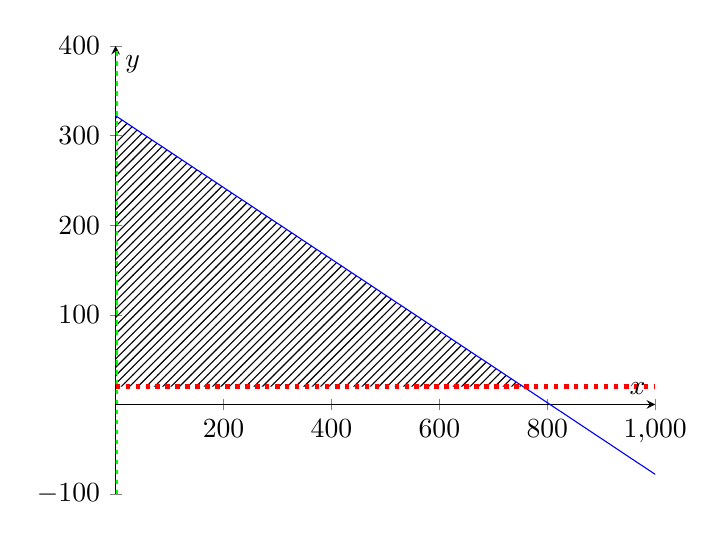
\begin{tikzpicture}
      \begin{axis}[
        xmin = 0, xmax = 1000,
        ymin = -100, ymax = 400,
        axis lines = center,
        xlabel = $ x $,
        ylabel = $ y $
      ]
        \addplot[domain = 0:1000, color = blue, samples=100, name path = TOP] {0.2*(1610 - 2*x)};
        \addplot +[mark=none, color = green, dotted, ultra thick] coordinates {(0, -100) (0, 400)};
        \addplot[domain = 0:1000, color = red, samples=100, dotted, ultra thick, name path = BOTTOM] {20};
        \addplot[gray, pattern=north east lines] fill between[of=TOP and BOTTOM, soft clip={domain=0:755}];
      \end{axis}
    \end{tikzpicture}}
  \end{center}

  In diagrams, we use dotted lines for strict inequalities ($ < $ and $ > $), and solid lines for normal inequalities ($ \geq $ and $ \leq $).
  The the set of all points $ (x,y) $ that satisfy every inequality in the system is called the \df{feasible region}; we have shaded it in the
  above diagram.
\end{ex}

We should also state the following definition and theorem for the sake of completeness.
\begin{defn}
  We write that $ x \geq y $ if there exists some non-negative real number $ a $ such that $ x = y + a $. If $ a \neq 0 $,
  then we write $ x > y $.
\end{defn}

\begin{thm}
  Suppose that $ x \geq y $.
  \begin{enumerate}
    \item If $ y \geq z $, then $ x \geq z $.
    \item If $ r $ is any real number, then $ x + r \geq y + r $.
    \item If $ \lambda $ is any \emph{positive} real number, then $ \lambda x \geq \lambda y $.
    \item If $ \lambda $ is any \emph{negative} real number, then $ \lambda y \geq \lambda x $.
  \end{enumerate}
\end{thm}
\begin{proof}
  One at a time:
  \begin{enumerate}
    \item We have $ x = y + a $ and $ y = z + b $ (for non-negative $ a $ and $ b $), so $ x = z + (a + b) $ and $ x \geq z $.
    \item We have $ x = y + a $ so $ x + r = (y + r) + a $ and $ x + r \geq y + r $.
    \item We have $ x = y + a $ so $ \lambda x = \lambda y + (\lambda a) $. Since both $ \lambda $ and $ a $ are nonnegative, their
          product is nonnegative; hence $ \lambda x \geq \lambda y $.
    \item We have $ x = y + a $ so $ \lambda x = \lambda y + (\lambda a) $, where $ \lambda a $ is nonpositive; hence $ -\lambda a $ is
          nonnegative, and $ \lambda x + (-\lambda a) = \lambda y $ implies that $ \lambda y \geq \lambda x $.
  \end{enumerate}
\end{proof}

There is not much else to say about systems of linear inequalities with as little structure as those we have seen in this section; we can
find the `corners' of the system by solving the corresponding system of linear equations, we can check if a point is within the feasible
region, and that's about it.

Final note: for each system of linear inequalities, we have a corresponding system of linear equalities obtained by replacing each inequality
sign with an equality sign.

\subsection*{Exercises}
\begin{enumerate}
  \item Write down the linear constraints corresponding to the following situations, and graph the feasible regions.
    \begin{enumerate}
      \item Hayden is taking a mathematics exam and needs to complete at least ten geometry problems and algebra problems within three hours. It
            will take him thirty minutes to complete a geometry problem and ten minutes to complete an algebra problem.
      \item Fuel from petrol pump A costs \$2.19 per litre and from petrol pump B costs \$1.69 per litre. Richard Seddon has at most \$20 to spend on fuel.
      \item John is packing apples and oranges into boxes. Each box can hold either 15 apples or 8 oranges. He needs to pack at least 40 boxes and
            at least 360 pieces of fruit.
    \end{enumerate}
  \item During a family trip, Andr\'e Weil shared the driving with his father. At most, he was allowed to drive for three hours in total. While driving, his
        maximum speed was eighty kilometres per hour. Write a system of inequalities describing the possible number of hours $ t $ and distance $ d $ that
        he may have driven; is it possible that he drove for 160 kilometres?
\end{enumerate}

\section{Linear Programming}
We can introduce some additional structure to a linear inequalities problem by adding an additional constraint: suppose we want to find the point
within the feasible region that maximises or minimises some other quantity.

\begin{ex}
  A company produces two models of sewing machine. Each unit of model A requires four hours of work on the first assembly line, and five on
  the second; each unit of model B requires seven hours of work on the first line, but only three on the second. During a week, the first line
  is allowed to spend up to 160 man-hours on sewing machines, and the second line is allowed to spend up to 80 man-hours on sewing machines. The
  total profit resulting from the sale of a single unit of model A is \$60; the total profit resulting from the sale of a unit of model B is \$50.
\end{ex}

In this case the quantity to be maximised is the profit, given by the function
\begin{equation}
  \theta(a,b) = 60a + 50b,
\end{equation}
where $ a $ is the total number of model A units produced, and $ b $ is the total number of model B units produced. We call a constraint function
such as this an \df{objective function}.

Our main result is the following theorem.
\begin{thm}[Main Theorem on Linear Inequalities, two variable case]
  Consider any system of linear inequalities in two variables $ x $ and $ y $ and any linear objective function $ \theta(x,y) $. Then the maximum
  and minimum values of $ \theta $ occur at the `corners' of the linear system; that is, the intersection points of the individual linear functions
  of the system.
\end{thm}
We will postpone the proof of this theorem to a later section as it is a little technical (in fact, we prove it in the general $ n $ variable case).
However, we can look at a simple example to convince ourselves that it is reasonable.

\begin{ex}\label{ex:linprog2d}
  Consider the following system; it does not matter precisely what the actual linear inequations are. Suppose that we wish
  to maximise the value $ C $ given by some linear equation $ ax + by = C $. Let us graph this situation for different values of $ C $:

  \begin{center}
    \fbox{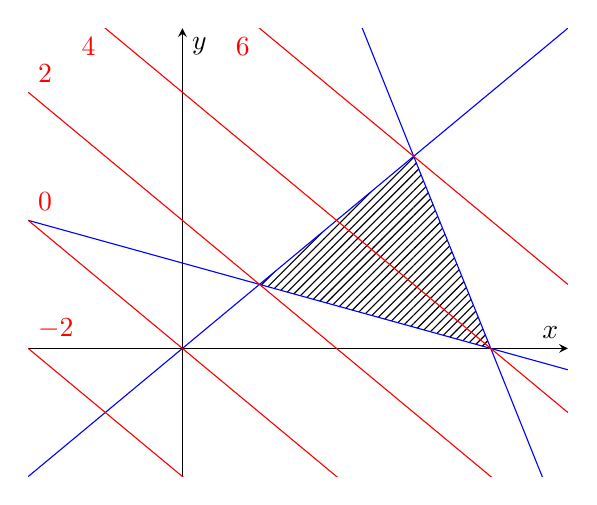
\begin{tikzpicture}
      \begin{axis}[
        xmin = -2, xmax = 5,
        ymin = -2, ymax = 5,
        xticklabels = {,,},
        yticklabels = {,,},
        ticks=none,
        axis lines = center,
        xlabel = $ x $,
        ylabel = $ y $
      ]
        \addplot[domain = -2:5, color = blue, samples=100, name path = TOP_LEFT] {x};
        \addplot[domain = -2:5, color = blue, samples=100, name path = TOP_RIGHT] {-3*x + 12};
        \addplot[domain = -2:5, color = blue, samples=100, name path = BOTTOM] {-(1/3)*(x - 1) + 1};
        \addplot[gray, pattern=north east lines] fill between[of=TOP_LEFT and BOTTOM, soft clip={domain=1:3}];
        \addplot[gray, pattern=north east lines] fill between[of=TOP_RIGHT and BOTTOM, soft clip={domain=3:4}];

        \addplot[domain = -2:5, color = red, samples=100] {-x - 2};
        \addplot[domain = -2:5, color = red, samples=100] {-x};
        \addplot[domain = -2:5, color = red, samples=100] {-x + 2};
        \addplot[domain = -2:5, color = red, samples=100] {-x + 4};
        \addplot[domain = -2:5, color = red, samples=100] {-x + 6};
        \node[above right, red] at (-2,0) {$ -2 $};
        \node[above right, red] at (-2,2) {$ 0 $};
        \node[above right, red] at (-2,4) {$ 2 $};
        \node[below left, red] at (-1,5) {$ 4 $};
        \node[below left, red] at (1,5) {$ 6 $};
      \end{axis}
    \end{tikzpicture}}
  \end{center}

  Since an increase in $ C $ means either in increase or a decrease in the $ y$-intercept of $ C = ax + by $ (depending on the sign of $ a $ and $ b $) but
  no change of slope of the function, it follows that the highest value of $ C $ such that $ ax + by = C $ still passes through the feasible region causes
  the function to pass through one of the corners of the feasible region.
\end{ex}

\begin{figure}
  \centering
  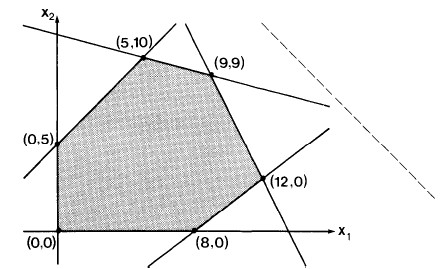
\includegraphics[width=0.5\textwidth]{progexample}
  \caption{Yet another feasible region.\label{fig:progexample}}
\end{figure}

\begin{ex}
  Consider the linear programming scenario pictured in figure \ref{fig:progexample}. Suppose we have further been given
  an objective function $ f(x,y) = 3x - 4y $. By the main theorem on linear programming, the maximum and minimum values
  of $ f $ must occur at corners. The maximum value, for example, occurs at $ (12,0) $.
\end{ex}

Since this topic is perhaps the most boring of all the L3 mathematics topics, we will not dwell further on it. If the reader is a
computer scientist and is expecting a general algorithm for solving linear programs like that given earlier for linear systems of
equations, she is advised to either search for `simplex algorithm' or to study a real subject.

\subsection*{Exercises}
\begin{enumerate}
  \item A manufacturer produces two different models, $ X $ and $ Y $, of the same product. There are two different raw materials, $ m $ and $ n $,
        required for each model. At least 18 units of raw material $ m $ and 12 units of raw material $ n $ must be used per day. There are at most
        34 hours of labour allowed each day. For model $ X $, 2 units of $ m $ and 1 of $ n $ is required; for model $ Y $, 1 unit of each is required.
        It requires 3 hours to manufacture one model $ X $ unit, and 2 hours to manufacture one model $ Y $ unit. The profit is \$3 for each model $ X $,
        and \$5 for each model $ Y $. How many units of each model should be produced each day to maximise the profit?
  \item Before opening a new factory, the following information (based on a single hour of operation) is considered.
        \begin{center}
          \begin{tabular}{lccc}
            & \textbf{\shortstack{No. of Type I\\Produced}} & \textbf{\shortstack{No. of Type II\\Produced}} & \textbf{\shortstack{Sulfur Oxides\\Released (kg)}}\\\hline
            Prod. Line A & 10 & 20 & 3\\
            Prod. Line B & 10 & 30 & 5\\\hline
          \end{tabular}
        \end{center}
        The factory must produce at least 50 units of type I and at least 120 of type II per hour. How many of each type of production line
        should be installed to minimise the amount of sulfur oxides released?
  \item A company produces boxes of pens and of pencils. There is an expected demand of at least 100 boxes of pens and 80 boxes of pencils
        each day. No more than 200 boxes of pens and 170 boxes of pencils can be made daily, but a total of at least 200 boxes must be shipped
        each day. If each box of pens sold results in a \$1 loss, but each box of pencils produces a \$2 profit, how many of each type should be made daily?
\end{enumerate}

\section{Linear Inequalities in $ n $ Variables}
Our results also apply naturally to higher-dimensional cases.
\begin{ex}[Scholarship 2016]
  A student is to sit an examination. The questions are divided into three groups. The student may
  answer any question from any group so long as the total number of questions answered does not
  exceed 100. The groups are characterised as follows:
  \begin{itemize}
    \item Group 1 --- easy, worth four marks each, and will take an average time of two minutes per
          question to answer.
    \item Group 2 --- moderate difficulty, worth five marks each, and will take an average time of three
          minutes per question to answer.
    \item Group 3 --- the most difficult, worth six marks each, and will take an average time of four
          minutes per question to answer.
  \end{itemize}
  The total time available to the student is 3.5 hours. The questions in groups 1 and 2 are the most mechanical
  and the student can tolerate only 2.5 hours of this kind of work before losing motivation.

  What combination of questions should the student answer for a maximum grade, assuming all answered questions are correct?
\end{ex}

Instead of having a feasible region that is geometrically a plane region, we now have a feasible region that is a volume. Our constraints
are (in three variables each):
\begin{gather}
  2x_1 + 3x_2 + 4x_3 \leq 210, \tag{L1} \\
  2x_1 + 3x_2 \leq 150, \tag{L2} \\
  x_1 + x_2 + x_3 \leq 100, \tag{L3} \\
  x_1 \geq 0, \tag{L4} \\
  x_2 \geq 0, \text{ and} \tag{L5}\\
  x_3 \geq 0. \tag{L6}
\end{gather}
Each represents a plane in 3-space.

Our objective function is
\begin{equation}
  G = 4x_1 + 5x_2 + 6x_3.
\end{equation}

Since we are in three dimensions, a `corner' is now the intersection point of three (or more) of our constraint
surfaces. Since we have 6 constraint surfaces, there are at most $ \binom{6}{3} = 20 $ corners.

\begin{figure}
  \centering
  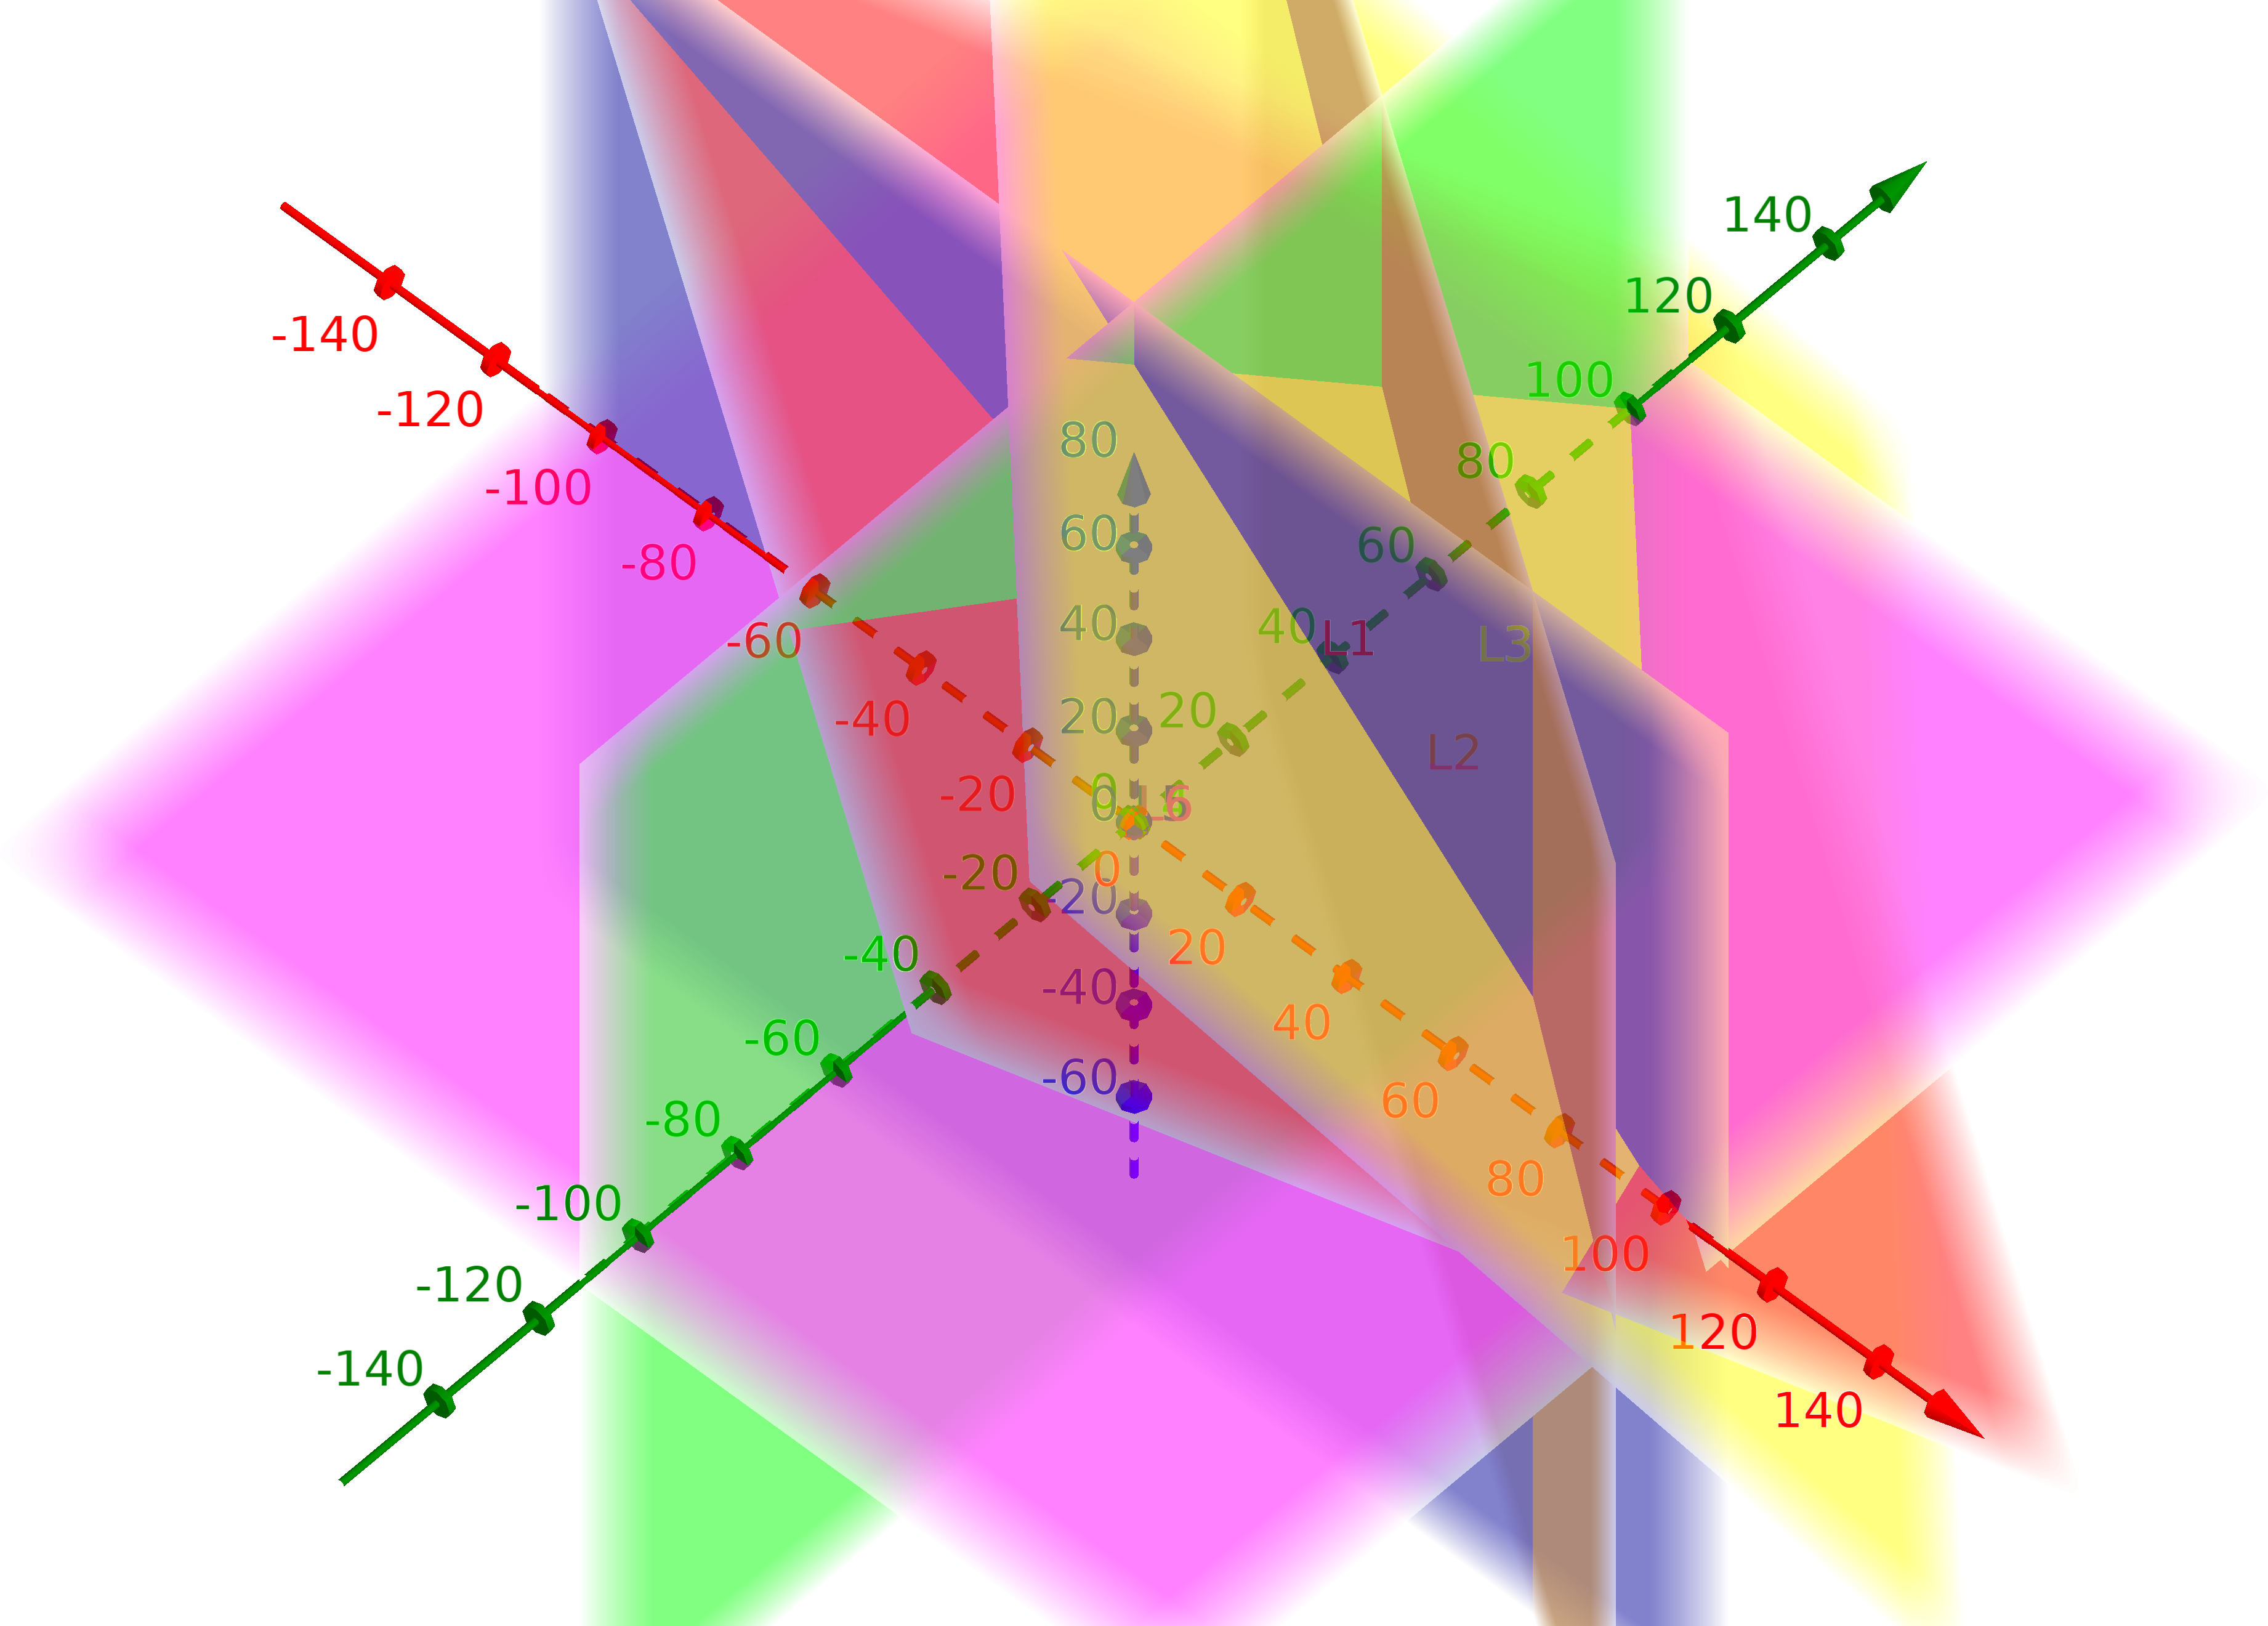
\includegraphics[width=0.7\textwidth]{linprog3d}
  \caption{The inequations L1-6 correspond to red, orange, yellow, green, blue, and pink respectively.\label{fig:linprog3d}}
\end{figure}

If we do this, we find 18 corners (combinations) --- there are two missing, since the combinations of L1/L2/L6, and L2/L4/L5 are
inconsistent (the three planes do not meet in either case). By drawing a suitable diagram of the situation (figure \ref{fig:linprog3d}),
it is possible to minimise the amount of further work required by throwing out all the other corners that miss out on being within
the feasible region.

Table \ref{tab:linprog3d} shows the final results. Hence, for the highest grade (of 390) the student should answer 75 questions from
group 1, none from group 2, and 15 from group 3.

\begin{table}
  \centering
  \begin{tabular}{cccc}
    \textbf{Planes} & \textbf{Corner} & \textbf{Feasible?} & \textbf{Objective function}\\\hline
    L1/L2/L3 & $ (105, -20, 15)$ & No & N/A\\
    L1/L2/L4 & $ (0,50,15) $ & Yes & 340 \\
    L1/L2/L5 & $ (75,0,15) $ & Yes & 390 \\
    L1/L2/L6 & inconsistent & No & N/A\\
    L1/L3/L4 & $ (0,190,-90) $ & No & N/A\\
    L1/L3/L5 & $ (95,0,5) $ & No & N/A \\
    L1/L3/L6 & $ (90,10,0) $ & No & N/A \\
    L1/L4/L5 & $ (0,0,52.5) $ & Yes & 315 \\
    L1/L4/L6 & $ (0,70,0) $ & No & N/A \\
    L1/L5/L6 & $ (105,0,0) $ & No & N/A \\
    L2/L3/L4 & $ (0,50,50) $ & No & N/A \\
    L2/L3/L5 & $ (75,0,25) $ & No & N/A \\
    L2/L3/L6 & $ (150,-50,0) $ & No & N/A\\
    L2/L4/L5 & inconsistent & No & N/A\\
    L2/L4/L6 & $ (0,50,0) $ & Yes & 250 \\
    L2/L5/L6 & $ (75,0,0) $ & Yes & 300 \\
    L3/L4/L5 & $ (0,0,100) $ & No & N/A \\
    L3/L4/L6 & $ (0,100,0) $ & No & N/A \\
    L3/L5/L6 & $ (100,0,0) $ & No & N/A \\
    L4/L5/L6 & $ (0,0,0) $ & Yes & 0
  \end{tabular}
  \caption{\label{tab:linprog3d}}
\end{table}

\subsection*{Exercises}
\begin{enumerate}
  \item Draw a picture analagous to that in example \ref{ex:linprog2d} for the 3D case.
  \item Maximise the function $ z = 2x_1 + x_2 + 2x_4 $, subject to
        \begin{displaymath}
          \begin{cases}
             x_1 + 2x_2 - x_3 &\geq 5\\
             x_2 + x_3 + x_4 &\leq 12\\
             2x_1 - x_2 - 3x_3 - 2x_4 &\leq -10\\
             x_j &\geq 0 \text{ for each } j = 1,...,4.
          \end{cases}
        \end{displaymath}
\end{enumerate}

\section{Proof of the Main Theorem on Linear Inequalities}
\begin{center}
  \emph{An engineer hears that a famous mathematician will be giving a public lecture, and always having a soft spot for math,
        he attends. The mathematician then talks at length about all sorts of amazing phenomena that happen in 17 dimensional space.
        The engineer, amazed at this mathematician's intuition for 17 dimensional space, goes up to him afterwards and asks `How do you
        picture 17 dimensions?'; the mathematician answers, `Oh, it's easy. Just imagine $n$-dimensional space, and set $n$ to 17.'}
\end{center}
The goal of this section is to state and prove in full generality the main theorem on linear inequalities. It may be safely skipped.

We need a small geometric definition:
\begin{defn}\leavevmode
  \begin{enumerate}
    \item A \textbf{closed half-space} of $ n $ dimensions is the set of all points $ (x_1, \dots, x_n) $ satisfying some linear
          inequality $ a_1 x_1 + \cdots + a_n x_n \leq b $.
    \item The \textbf{boundary} of the closed half-space $ a_1 x_1 + \cdots + a_n x_n \leq b $ is the set of all points
          satisfying $ a_1 x_1 + \cdots + a_n x_n = b $.
    \item A \textbf{convex polytope} of $ n $ dimensions is an intersection of a finite number of closed half-spaces of $ n $ dimensions.
    \item A point $ x$ is an \textbf{interior point} of a complex polytope $ P $ if there exists some real number $ \varepsilon > 0 $ such that the sphere
          of radius $ \varepsilon $ centred at $ x $ is contained entirely within $ P $.
    \item A convex polytope $ P $ is \textbf{bounded} if there exists some real number $ \varepsilon > 0 $ such that every point of $ P $ is contained within
          the sphere of radius $ \varepsilon $  centred at the origin. (Intuitively, $ P $ does not go ``to infinity''.)
    \item A \textbf{face} of a convex polytope $ P $ is any intersection of $ P $ with a closed half-space such that none of the interior points of $ P $
          lie on the boundary of the half-space.
    \item A \textbf{vertex} of a convex polytope is a 0-dimensional face.
  \end{enumerate}
\end{defn}

\begin{ex}
  A convex polygon is a convex polytope of two dimensions; a convex polyhedra is a convex polytope of three regions. In general, the
  feasible region of some system of linear inequalities is a convex polytope.
\end{ex}

\begin{thm}[Main Theorem on Linear Inequalities]
  Let $ \theta $ be a linear function in $ n $ variables, and let $ P $ be a bounded polytope of $ n $ dimensions. Suppose that there is some point $ x^* $
  in $ P $ such that for all $ x $ in $ P $, $ \theta(x) \leq \theta(x^*) $. Then $ x^* $ is either a vertex of $ P $, or lies in a face of $ P $ such that
  for every point $ x' $ in that face (in particular, including the vertices of that face) we have $ \theta(x') = \theta(x^*) $.
\end{thm}
\begin{proof}
  Let $ \theta(y_1, \dots, y_n) = a_1 y_1 + \cdots + a_n y_n $, and let $ x^* = (x_1, \dots, x_n ) $. Suppose that $ x^* $ is in the interior
  of $ P $ (i.e. $ x^* $ is not in any face of $ P $). Then there exists some $ \varepsilon > 0 $ such that the sphere $ S $ of radius $ \varepsilon $ centred
  at $ x^* $ is contained entirely within $ P $. Note that the point
  \begin{displaymath}
    x^\dagger = (x_1 - \frac{\varepsilon}{2} \frac{a_1}{\sqrt{a_1^2 + \cdots + a_n^2}}, \dots, x_n - \frac{\varepsilon}{2} \frac{a_n}{\sqrt{a_1^2 + \cdots + a_n^2}})
  \end{displaymath}
  is still contained within $ S $ and hence within $ P $, because the distance between $ x^* $ and $ x^\dagger $ is less than $ \varepsilon $ (check this).

  Now consider
  \begin{align*}
    \theta(x^\dagger) &= a_1 x_1 - \frac{\varepsilon}{2} \frac{a_1^2}{\sqrt{a_1^2 + \cdots + a_n^2}} + \dots
                       + a_n x_n - \frac{\varepsilon}{2} \frac{a_n^2}{\sqrt{a_1^2 + \cdots + a_n^2}}\\
                      &= a_1 x_1 + \cdots + a_n x_n - \frac{\varepsilon}{2} \sqrt{a_1^2 + \cdots + a_n^2}\\
                      &= \theta(x^*) - \frac{\varepsilon}{2} \sqrt{a_1^2 + \cdots + a_n^2}.
  \end{align*}
  But recall that $ \varepsilon > 0 $; so in particular, $ \frac{\varepsilon}{2} \sqrt{a_1^2 + \cdots + a_n^2} > 0 $. So the value of $ \theta(x^\dagger) $ is
  less than that of $ \theta(x^*) $; this is a contradiction and so $ x^* $ lies on a face of $ P $.

  Now, suppose that $ x^* $ lies on a face of $ P $ that is not a vertex. Suppose that the face is $ m$-dimensional. Then we have a minimum value of $ \theta $ on
  the inside of a $ m$-dimensional polytope, which is a contradiction unless $ \theta $ is constant on the face; hence the minimum value also occurs on the boundaries
  of this face. We can repeat this argument for the boundaries (which will be polytopes of dimension less than $ m $), and in particular in at most $ m-1 $ steps
  will reach a polytope of only one dimension; one final application of the proof above shows that $ x^* $ must occur on a vertex of the original polytope, and we
  are done.
\end{proof}

\subsection*{Exercises}
\begin{enumerate}
  \item Explain why a half-space is called a half-space.
  \item Draw a tetrahedron and indicate the 0-, 1-, and 2-dimensional faces.
  \item Show that $ x^\dagger $ is still in $ S $.
  \item Note that we only proved the theorem for placing the \emph{minimum} value of our objective function on a vertex of our feasible
        region. Show that placing the maximum value on a vertex is an easy consequence of this. [Hint: consider $ -\theta $.]
\end{enumerate}

\section{More Exercises}
\begin{center}
  \emph{Mr. Sun came out and he smiled at me\\Said, ``It's gonna be a good one, just wait and see''}\\--- Spongebob Squarepants, S4E20
\end{center}
\begin{enumerate}
  \item For each of the following, describe the system graphically and solve if possible.
    \begin{center}
      \hspace*{\fill}\begin{enumerate*}
        \item
          $ \displaystyle
            \begin{cases}
              2x + 3y = 6\\
              9x + 2y = 19\\
              4x + 6y = 14.
            \end{cases}
          $\hspace*{\fill}
        \item
          $ \displaystyle
            \begin{cases}
              x + 2y + z = 6\\
              2x - y + z = 8\\
              -2x + y + z = 4.
            \end{cases}
          $\hspace*{\fill}
        \item
          $ \displaystyle
            \begin{cases}
              x + y + z = 3\\
              x + y + z = 4\\
              x - y + z = 3\\
              -x + y -z = 4
            \end{cases}
          $\hspace*{\fill}
      \end{enumerate*}
    \end{center}
  \item Find the row-reduced echelon form of each of the following matrices, and write down the corresponding systems of equations.
    \begin{center}
      \hspace*{\fill}\begin{enumerate*}
        \item $ \displaystyle\begin{bmatrix}[ccc|c] 1 & 2 & 0 & 1\\0 & 0 & 1 & 16 \end{bmatrix} $\hspace*{\fill}
        \item $ \displaystyle\begin{bmatrix}[cc|c] 3 & 1 & 4\\1 & 5 & 9\\2 & 6 & 5 \end{bmatrix} $\hspace*{\fill}
        \item $ \displaystyle\begin{bmatrix}[cc|c] \sqrt{2} & \sqrt{3} & \sqrt{5} \\ 2 & 3 & 5 \\ 2^2 & 3^2 & 5^2 \end{bmatrix} $\hspace*{\fill}
      \end{enumerate*}
    \end{center}
  \item Compute $ \begin{vmatrix} 2 & 3\\3 & 2 \end{vmatrix} $ and $ \begin{vmatrix} 1 & 2 & 3 \\ 4 & 5 & 6 \\ 7 & 8 & 9 \end{vmatrix} $.
  \item Agatha and Arthur are buying cooking supplies. In total, they wish to buy 3 kilograms of flour and sugar. They
        have \$24 available; flour costs \$6 per kilogram, and sugar costs \$9 per kilogram. How much flour and sugar do they buy?
  \item Solve the following system.
        \begin{displaymath}
          \begin{cases}
          9^{2x+y} - 9^x \times 3^y = 6\\
          \log_{x+1}(y+3) + \log_{x+1}(y+x+4) = 3
          \end{cases}
        \end{displaymath}
  \item Explain why we cannot subtract true linear inequalities from each other to obtain another true linear inequality:
        \begin{align*}
          1 &\leq 2 \text{ and}\\
          4 &\leq 8 \text{ but}\\
          -3 &\not\leq -6.
        \end{align*}
        (This explains why we cannot simply solve linear programming problems by row reduction.)
  \item For each of the following, draw the feasible region.
    \begin{center}
      \hspace*{\fill}\begin{enumerate*}
        \item
          $ \displaystyle
            \begin{cases}
              2x + 3y \leq 6\\
              9x + 2y \geq 19\\
              4x + 6y < 14.
            \end{cases}
          $\hspace*{\fill}
        \item
          $ \displaystyle
            \begin{cases}
              x < y\\
              2x > 3\\
              y < 4
            \end{cases}
          $\hspace*{\fill}
        \item
          $ \displaystyle
            \begin{cases}
              x + y + 1 < 0\\
              2 - x > 6\\
              (x + 1)(y + 2) > 0
            \end{cases}
          $\hspace*{\fill}
      \end{enumerate*}
    \end{center}
  \item Come up with an example of a 2-variable linear programming problem involving a \emph{quadratic} objective function
        such that the objective function is maximised at a point inside the feasible region.
  \item A publisher has orders for 600 copies of a book from Wellington and 400 copies from Christchurch. The company has 700 copies in
        a warehouse in Dunedin and 800 copies in a warehouse in Auckland. It costs \$5 to ship a text from Dunedin to Christchurch, but
        it costs \$10 to ship it to Wellington. It costs \$15 to ship a text from Auckland to Christchurch, but it costs \$4 to ship it from
        Auckland to Wellington. How many copies should the company ship from each warehouse to Wellington and Christchurch to fill the
        order at the least cost?
  \item A company produces three items, A, B, and C. The company has three factories, each
        of which produces the three items in the quantities per hour indicated in the following table:
        \begin{center}
          \renewcommand{\arraystretch}{1.5}
          \begin{tabular}{  c | c | c | c | c | }
            \multicolumn{1}{r}{} & \multicolumn{1}{r}{} & \multicolumn{3}{c}{Plant} \\ \cline{3-5}
            \multicolumn{1}{r}{} & & \textit{I} & \textit{II} & \textit{III} \\ \cline{2-5}
            \multirow{3}{*}{Item} & \textit{A} & 1 & 2 & 3 \\ \cline{2-5}
            & \textit{B} & 2 & 1 & 4 \\ \cline{2-5}
            & \textit{C} & 3 & 1 & 1 \\ \cline{2-5}
          \end{tabular}
        \end{center}
        It costs \$1000 per hour to operate plant I, \$400 per hour
        to operate plant II, and \$2400 per hour to operate plant III.

        An order is placed with the company for three units of item A, five of item B,
        and six of item C. Determine the number of hours each plant should be operated
        to produce at least the required number of items for the order at minimum cost.
\end{enumerate}

\end{document}
